\documentclass[a4paper,11pt,oneside]{memoir}

% Castellano
\usepackage[spanish,es-tabla]{babel}
\selectlanguage{spanish}
\usepackage[utf8]{inputenc}
\usepackage{placeins}

\RequirePackage{booktabs}
\RequirePackage[table]{xcolor}
\RequirePackage{xtab}
\RequirePackage{multirow}

% Links
\usepackage[colorlinks]{hyperref}
\hypersetup{
	allcolors = {red}
}

% Ecuaciones
\usepackage{amsmath}

% Rutas de fichero / paquete
\newcommand{\ruta}[1]{{\sffamily #1}}

% Párrafos
\nonzeroparskip


% Imagenes
\usepackage{graphicx}
\newcommand{\imagen}[2]{
	\begin{figure}[!h]
		\centering
		\includegraphics[width=0.9\textwidth]{#1}
		\caption{#2}\label{fig:#1}
	\end{figure}
	\FloatBarrier
}

\newcommand{\imagenflotante}[2]{
	\begin{figure}%[!h]
		\centering
		\includegraphics[width=0.9\textwidth]{#1}
		\caption{#2}\label{fig:#1}
	\end{figure}
}



% El comando \figura nos permite insertar figuras comodamente, y utilizando
% siempre el mismo formato. Los parametros son:
% 1 -> Porcentaje del ancho de página que ocupará la figura (de 0 a 1)
% 2 --> Fichero de la imagen
% 3 --> Texto a pie de imagen
% 4 --> Etiqueta (label) para referencias
% 5 --> Opciones que queramos pasarle al \includegraphics
% 6 --> Opciones de posicionamiento a pasarle a \begin{figure}
\newcommand{\figuraConPosicion}[6]{%
  \setlength{\anchoFloat}{#1\textwidth}%
  \addtolength{\anchoFloat}{-4\fboxsep}%
  \setlength{\anchoFigura}{\anchoFloat}%
  \begin{figure}[#6]
    \begin{center}%
      \Ovalbox{%
        \begin{minipage}{\anchoFloat}%
          \begin{center}%
            \includegraphics[width=\anchoFigura,#5]{#2}%
            \caption{#3}%
            \label{#4}%
          \end{center}%
        \end{minipage}
      }%
    \end{center}%
  \end{figure}%
}

%
% Comando para incluir imágenes en formato apaisado (sin marco).
\newcommand{\figuraApaisadaSinMarco}[5]{%
  \begin{figure}%
    \begin{center}%
    \includegraphics[angle=90,height=#1\textheight,#5]{#2}%
    \caption{#3}%
    \label{#4}%
    \end{center}%
  \end{figure}%
}
% Para las tablas
\newcommand{\otoprule}{\midrule [\heavyrulewidth]}
%
% Nuevo comando para tablas pequeñas (menos de una página).
\newcommand{\tablaSmall}[5]{%
 \begin{table}
  \begin{center}
   \rowcolors {2}{gray!35}{}
   \begin{tabular}{#2}
    \toprule
    #4
    \otoprule
    #5
    \bottomrule
   \end{tabular}
   \caption{#1}
   \label{tabla:#3}
  \end{center}
 \end{table}
}

%
% Nuevo comando para tablas pequeñas (menos de una página).
\newcommand{\tablaSmallSinColores}[5]{%
 \begin{table}[H]
  \begin{center}
   \begin{tabular}{#2}
    \toprule
    #4
    \otoprule
    #5
    \bottomrule
   \end{tabular}
   \caption{#1}
   \label{tabla:#3}
  \end{center}
 \end{table}
}

\newcommand{\tablaApaisadaSmall}[5]{%
\begin{landscape}
  \begin{table}
   \begin{center}
    \rowcolors {2}{gray!35}{}
    \begin{tabular}{#2}
     \toprule
     #4
     \otoprule
     #5
     \bottomrule
    \end{tabular}
    \caption{#1}
    \label{tabla:#3}
   \end{center}
  \end{table}
\end{landscape}
}

%
% Nuevo comando para tablas grandes con cabecera y filas alternas coloreadas en gris.
\newcommand{\tabla}[6]{%
  \begin{center}
    \tablefirsthead{
      \toprule
      #5
      \otoprule
    }
    \tablehead{
      \multicolumn{#3}{l}{\small\sl continúa desde la página anterior}\\
      \toprule
      #5
      \otoprule
    }
    \tabletail{
      \hline
      \multicolumn{#3}{r}{\small\sl continúa en la página siguiente}\\
    }
    \tablelasttail{
      \hline
    }
    \bottomcaption{#1}
    \rowcolors {2}{gray!35}{}
    \begin{xtabular}{#2}
      #6
      \bottomrule
    \end{xtabular}
    \label{tabla:#4}
  \end{center}
}

%
% Nuevo comando para tablas grandes con cabecera.
\newcommand{\tablaSinColores}[6]{%
  \begin{center}
    \tablefirsthead{
      \toprule
      #5
      \otoprule
    }
    \tablehead{
      \multicolumn{#3}{l}{\small\sl continúa desde la página anterior}\\
      \toprule
      #5
      \otoprule
    }
    \tabletail{
      \hline
      \multicolumn{#3}{r}{\small\sl continúa en la página siguiente}\\
    }
    \tablelasttail{
      \hline
    }
    \bottomcaption{#1}
    \begin{xtabular}{#2}
      #6
      \bottomrule
    \end{xtabular}
    \label{tabla:#4}
  \end{center}
}

%
% Nuevo comando para tablas grandes sin cabecera.
\newcommand{\tablaSinCabecera}[5]{%
  \begin{center}
    \tablefirsthead{
      \toprule
    }
    \tablehead{
      \multicolumn{#3}{l}{\small\sl continúa desde la página anterior}\\
      \hline
    }
    \tabletail{
      \hline
      \multicolumn{#3}{r}{\small\sl continúa en la página siguiente}\\
    }
    \tablelasttail{
      \hline
    }
    \bottomcaption{#1}
  \begin{xtabular}{#2}
    #5
   \bottomrule
  \end{xtabular}
  \label{tabla:#4}
  \end{center}
}



\definecolor{cgoLight}{HTML}{EEEEEE}
\definecolor{cgoExtralight}{HTML}{FFFFFF}

%
% Nuevo comando para tablas grandes sin cabecera.
\newcommand{\tablaSinCabeceraConBandas}[5]{%
  \begin{center}
    \tablefirsthead{
      \toprule
    }
    \tablehead{
      \multicolumn{#3}{l}{\small\sl continúa desde la página anterior}\\
      \hline
    }
    \tabletail{
      \hline
      \multicolumn{#3}{r}{\small\sl continúa en la página siguiente}\\
    }
    \tablelasttail{
      \hline
    }
    \bottomcaption{#1}
    \rowcolors[]{1}{cgoExtralight}{cgoLight}

  \begin{xtabular}{#2}
    #5
   \bottomrule
  \end{xtabular}
  \label{tabla:#4}
  \end{center}
}


















\graphicspath{ {./img/} }

% Capítulos
\chapterstyle{bianchi}
\newcommand{\capitulo}[2]{
	\setcounter{chapter}{#1}
	\setcounter{section}{0}
	\chapter*{#2}
	\addcontentsline{toc}{chapter}{#2}
	\markboth{#2}{#2}
}

% Apéndices
\renewcommand{\appendixname}{Apéndice}
\renewcommand*\cftappendixname{\appendixname}

\newcommand{\apendice}[1]{
	%\renewcommand{\thechapter}{A}
	\chapter{#1}
}

\renewcommand*\cftappendixname{\appendixname\ }

% Formato de portada
\makeatletter
\usepackage{xcolor}
\newcommand{\tutor}[1]{\def\@tutor{#1}}
\newcommand{\course}[1]{\def\@course{#1}}
\definecolor{cpardoBox}{HTML}{E6E6FF}
\def\maketitle{
  \null
  \thispagestyle{empty}
  % Cabecera ----------------
\noindent
\includegraphics[width=\textwidth]{cabecera}\vspace{1cm}%
  \vfill
  % Título proyecto y escudo informática ----------------
  \colorbox{cpardoBox}{%
    \begin{minipage}{.8\textwidth}
      \vspace{.5cm}\Large
      \begin{center}
      \textbf{TFG del Grado en Ingeniería Informática}\vspace{.6cm}\\
      \textbf{\LARGE\@title{}}
      \end{center}
      \vspace{.2cm}
    \end{minipage}

  }%
  \hfill\begin{minipage}{.20\textwidth}
    
\includegraphics[width=\textwidth]{escudoInfor}
  \end{minipage}
  \vfill
  % Datos de alumno, curso y tutores ------------------
  \begin{center}%
  {%
    \noindent\LARGE
    Presentado por \@author{}\\ 
    en Universidad de Burgos --- \@date{}\\
    Tutor: \@tutor{}\\
  }%
  \end{center}%
  \null
  \cleardoublepage
  }
\makeatother

\newcommand{\nombre}{Nombre del alumno} %%% cambio de comando

% Datos de portada
\title{título del TFG}
\author{\nombre}
\tutor{nombre tutor}
\date{\today}

\begin{document}

\maketitle


\newpage\null\thispagestyle{empty}\newpage


%%%%%%%%%%%%%%%%%%%%%%%%%%%%%%%%%%%%%%%%%%%%%%%%%%%%%%%%%%%%%%%%%%%%%%%%%%%%%%%%%%%%%%%%
\thispagestyle{empty}


\noindent
\includegraphics[width=\textwidth]{cabecera}\vspace{1cm}

\noindent D. nombre tutor, profesor del departamento de nombre departamento, área de nombre área.

\noindent Expone:

\noindent Que el alumno D. \nombre, con DNI dni, ha realizado el Trabajo final de Grado en Ingeniería Informática titulado título de TFG. 

\noindent Y que dicho trabajo ha sido realizado por el alumno bajo la dirección del que suscribe, en virtud de lo cual se autoriza su presentación y defensa.

\begin{center} %\large
En Burgos, {\large \today}
\end{center}

\vfill\vfill\vfill

% Author and supervisor
\begin{minipage}{0.45\textwidth}
\begin{flushleft} %\large
Vº. Bº. del Tutor:\\[2cm]
D. nombre tutor
\end{flushleft}
\end{minipage}
\hfill
\begin{minipage}{0.45\textwidth}
\begin{flushleft} %\large
Vº. Bº. del co-tutor:\\[2cm]
D. nombre co-tutor
\end{flushleft}
\end{minipage}
\hfill

\vfill

% para casos con solo un tutor comentar lo anterior
% y descomentar lo siguiente
%Vº. Bº. del Tutor:\\[2cm]
%D. nombre tutor


\newpage\null\thispagestyle{empty}\newpage




\frontmatter

% Abstract en castellano
\renewcommand*\abstractname{Resumen}
\begin{abstract}
En este primer apartado se hace una \textbf{breve} presentación del tema que se aborda en el proyecto.
\end{abstract}

\renewcommand*\abstractname{Descriptores}
\begin{abstract}
Palabras separadas por comas que identifiquen el contenido del proyecto Ej: servidor web, buscador de vuelos, android \ldots
\end{abstract}

\clearpage

% Abstract en inglés
\renewcommand*\abstractname{Abstract}
\begin{abstract}
A \textbf{brief} presentation of the topic addressed in the project.
\end{abstract}

\renewcommand*\abstractname{Keywords}
\begin{abstract}
keywords separated by commas.
\end{abstract}

\clearpage

% Indices
\tableofcontents

\clearpage

\listoffigures

\clearpage

\listoftables
\clearpage

\mainmatter
\capitulo{1}{Introducción}

Este proyecto nació con el objetivo de llevar Thoth a la web usando para ello tecnologías adaptadas y que puedan ser utilizadas en diferentes dispositivos haciéndolo accesible a todo el mundo. Con ayuda de la herramienta conocida como GWT o Google Web Toolkit según su denominación inglesa, traduciré la aplicación a Javascript en el lado del cliente proporcionando un mejor funcionamiento dentro de los navegadores web.

Que es Thoth
Thoth es un antiguo proyecto enfocado a la actividad docente y relacionado con los procesadores de lenguaje, que fue realizado por varios alumnos de la Universidad de Burgos como trabajo de fin de carrera. Esta aplicación cuenta con dos versiones  hasta la fecha y con otros desarrollos como Web Thoth. informacion sobre ellos y enlace a la web. (Hay mas?)

Una de las principales preguntas que nos podemos hacer al ver este proyecto es el porqué traducir la aplicación al lenguaje JavaScript. 
En primer lugar todos los navegadores actuales son capaces de interpretar el código escrito en JavaScript y soportan al menos alguna de las versiones ECMAScript, siendo la última la sexta edición disponible desde 2015. Con ayuda de la tecnología AJAX, entre otras, este lenguaje es capaz de establecer comunicación cliente-servidor, algo que al principio de su desarrollo no lograba hacer. 

Porque utilizo GWT
Utilizo GWT para este proyecto como herramienta para desarrollar la aplicación. Pese a que actualmente no es el mejor <<framework>> para desarrollar si es una de las bases de otros mucho más modernos y potentes. La forma de trabajar con <<Google Web Toolkit>> es creando el código en Java y el compilador hará una traducción a los lenguajes JavaScript y HTML.

La elección surgió como un desafío para nosotros ya que otras herramientas el esfuerzo era mínimo. Este desafío consiste en que GWT no es capaz de admitir todas las librerías de Java y por eso debimos reescribir el código adaptándolo a las capacidades de este <<framework>> ((((Completar? que otras herramientas hay etc))))
\capitulo{2}{Objetivos del proyecto}

El objetivo principal de este trabajo de final de grado consiste en transformar el proyecto previo de Thoth, que está escrito en Java, a la tecnología web JavaScript. Esta conversión se llevará a cabo por medio de GWT, herramienta elegida posteriormente a un estudio previo (disponible en el capítulo Técnicas y Herramientas). 

El desarrollo consiste en una página web dinámica que sea capaz de hacer las mismas funcionalidades sobre gramáticas formales y sus algoritmos que en Thoth, poniendo a prueba mis propios conocimientos sobre Java así como otros lenguajes sobre tecnologías web como son HTML, CSS o JavaScript.

Pero el por qué pretendemos pasar de una aplicación de escritorio a otra que se ejecuta en el navegador es básicamente porque no es necesario instalar o descargar material para poderla utilizar Thoth, simplemente algunos conocimientos básicos sobre gramáticas formales. Por lo tanto aporta una clara ventaja con respecto a aplicaciones denominadas <<de escritorio>> como es el Thoth original sobre el que nos basamos en este proyecto.

La conversión de Thoth a GWT es necesaria porque amplía las posibilidades de mejora de las anteriores versiones. Pretendemos aportar mayor funcionalidad debido a que al ser una aplicación web podemos hacer un registro de los usuarios, con inicio de sesión, registro de actividades, etc. 

De hecho, uno de los puntos fuertes de este proyecto consiste en aprovechar la mayor parte de utilidad de las aplicaciones web. Aunque en las anteriores versiones la pretensión era sobre todo didáctica en materia relacionada con el estudio de los procesos del lenguaje, ahora además de eso también queremos llegar a poder saber la utilidad que se le da a Thoth. Para ello gracias al registro de información sobre los usuarios podremos saber cuando se ha registrado alguien, o iniciado sesión, qué gramáticas ha usado y más funcionalidades que puedan surgir. Eso si, siempre manteniendo la privacidad del usuario, cifrando la contraseña de registro.

Por último objetivo está el de experimentar con herramientas que no conocemos, y de esta forma ir aprendiendo a solucionar problemas nuevos. Al fin y al cabo lo que se trata de aprender en la universidad es a aprender a superar estos retos por uno mismo, aplicando las técnicas que se nos enseñan.

Los objetivos del proyecto quedan reflejados de esta manera:

\begin{itemize}

\item Estudio de aplicaciones de conversión automatica de Java a la web.
\item Convertir la parte de las gramáticas de Thoth mediante GWT
\item Crear un sistema de registro de usuarios para el acceso a la aplicación.
\item Crear un sistema de sesiones de acuerdo al registro.

\end{itemize}

\capitulo{3}{Conceptos teóricos}

En mi experiencia como profesor de programación, diseño 3D y robótica para alumnos de primaria, lo primero que les enseñábamos era a definir la programación como el lenguaje de comunicación entre nosotros, los humanos, y los ordenadores o los robots. Todo esto pertenece a los conceptos más puramente teóricos sobre la computación y que es, en sí, la base de la informática. 

Pues bien, a <<grosso modo>> el concepto es el mismo ahora. Como cada uno, hombre y máquina, <<habla>> un idioma diferente se debe establecer un lenguaje que sea la vía de comunicación entre ambos. 

Para poder entender todo lo que se va a tratar a continuación, debo explicar primero el concepto de \textit{autómata} o \textit{máquina abstracta}. Un autómata es un modelo matemático o un dispositivo teórico que recibe una cadena de símbolos como entrada y que al procesarla, genera un cambio de estado produciendo una salida determinada. Esta salida pude reconocer palabras y determinar si la entrada pertenece a un determinado lenguaje o no. En el símil anterior digamos que es el corrector, que cuando escribe el humano algo determina si esta bien escrito o no porque no lo va a poder entender el ordenador. 

Entonces ya sabemos que para que haya comunicación entre un ordenador o robot y un humano, tiene que haber un lenguaje y un autómata. Pero también algo más: una gramática.

\section{¿Qué es una gramática y para qué sirve?}

Una gramática formal es un mecanismo para la generación de cadenas de caracteres que son admitidas por un determinado lenguaje formal, y que utiliza un conjunto de reglas de formación. Por lo tanto, podemos entenderlo dentro del concepto de las ciencias de la computación y la lógica matemática. Las cadenas de caracteres resultantes son a su vez <<bien formadas>> cuando pertenecen al lenguaje formal con el que se trabaja \cite{aho1986compilers}.

¿Y porque es tan importante? Siguiendo con el ejemplo del principio, la gramática es la que va a determinar si lo que se introduce en el autómata es correcto o no. Un conjunto de reglas que nos indicará el por qué al juntar una serie de caracteres de una forma se van a poder entender.

Por otro lado, la denominación de la gramática formal desde un punto de vista más formal, de denomina como una cuádrupla compuesta por:

\begin{itemize}
	\item Un alfabeto de \textbf{símbolos terminales} o tókenes denominado con la letra griega $\Sigma$.
	\item $\mathcal{N}$ que es un alfabeto formado por \textbf{símbolos no terminales}.
	\item Un alfabeto de \textbf{producciones} denominado $\mathcal{P}$.
	\item Y por último un símbolo llamado \textbf{axioma} o símbolo inicial el cual $\mathcal{S} \in \mathcal{N}$.
\end{itemize}

El alfabeto total que compone la gramática esta formado, según lo anterior, por $\Sigma\cup\mathcal{N}$, es decir, por el conjunto de los símbolos terminales y no terminales.

Una \textbf{producción} tiene esta estructura y esta compuesto por un par ordenado de cadenas. \[x \rightarrow y\] A la parte izquierda se la denomina antecedente y la derecha es el consecuente. A las producciones también se las denomina reglas de derivación.

Pongamos un ejemplo de una gramática simple y veamos de que esta formada. Se suele utilizar el sistema de notación  \[x \rightarrow y\] \[z \rightarrow w\] para indicar una o varias producciones, en vez de \[(x, y) \in \mathcal{P} \] \[(z, w) \in \mathcal{P} \] siendo $\mathcal{P}$ el conjunto de producciones.

Por otro lado si hay más de una producción que comience con el mismo elemento la notación sería de esta forma \[ x \rightarrow y | z | w\] en lugar de ser \[ x \rightarrow y\] \[x \rightarrow z\] \[x \rightarrow w\].

Se denomina \textbf{derivación directa} cuando sea $x \rightarrow y$ una producción y $v, w \in \Sigma^{*}$ decimos que $w$ deriva directamente de $v$ ( $v \Rightarrow w$) si $\exists z, u \in \Sigma^{*}$ tales que $v=zxu, w=zyu$ y $x\rightarrow y$.

La \textbf{derivación}: sea $\Sigma$ un alfabeto, un conjunto de producciones de ese alfabeto denominada $\mathcal{P}$ y $v, w \in \Sigma^{*}$ decimos que $w$ deriva de $v$, si existen una cadena de derivación de longitud $n$ así $u_{0}, u_{1}, ..., u_{n} \in \Sigma^{*}$ tales que:
 \[ v = u_{0} \Rightarrow u_{1}\] \[ u_{1} \Rightarrow u_{2}\] \[...\] \[ u_{n-1} \Rightarrow u_{n} = w\]

Se habla de lenguaje generado por una gramática $G$ escrito así $L(G)$ y se define como el conjunto de todas las sentencias de la gramática $G$.  \[L(G) = x\in \Sigma^{*}:\mathcal{S} \Rightarrow^{+}x\]
De esta manera se dice que dos gramáticas son equivalentes $G_{1} \equiv G_{2}$ si generan el mismo lenguaje $L(G_{1})=L(G_{2})$.

\section{Recursividad}

Por último una gramática es recursiva en un símbolo no terminal $U$ cuando existe una forma sentencial de $U$ que contiene a $U$. \[U \Rightarrow^{+}xUy \textup{ donde } x,y\in (\Sigma \cup \mathcal{N})^{*} \]
Así pues la gramática será recursiva cuando lo sea para algún no terminal, si $x = \varepsilon$ la gramática es recursiva por la izquierda, y si $y = \varepsilon$ se dice que es recursiva por la derecha.

\section{Tipos de gramáticas }

Hay varios tipos de gramáticas según sus características.
\begin{itemize}
\item \textbf{Gramáticas de Chomsky}: las producciones tienen la forma \[u \rightarrow v \textup{ donde } u=xAy \in (\Sigma \cup \mathcal{N})^{+} \wedge A \in \mathcal{N} \wedge x, y, v \in (\Sigma \cup \mathcal{N})^{*}\]

Es posible demostrar que los lenguajes generados por una gramática de Chomsky de un grupo más restringido llamadas gramáticas con estructura de frase, es decir que ambas tienen la misma capacidad generativa. Las gramáticas de frase tienen la siguiente forma de producción:

\[xAy \rightarrow xvy \textup{ donde } x,y,v \in (\Sigma \cup \mathcal{N})^{*} \wedge A \in \mathcal{N}\]
\item \textbf{Gramaticas dependientes o sensibles al contexto}: Cuentas con las reglas de producción con forma  \[xAy \rightarrow xvy \textup{ donde } x, y \in (\Sigma \cup \mathcal{N})^{*} \wedge A \in \mathcal{N} \wedge v \in (\Sigma \cup \mathcal{N})^{+}\]
Este tipo de gramáticas el significado de $A$ depende del contexto o de la posición en la frase. El contexto sería entonces $x$ e $y$. La mayor parte de los lenguajes de ordenador pertenecen a este tipo. Además longitud de la parte derecha de las producciones es siempre mayor o igual que la de la parte izquierda.
\item \textbf{Gramáticas independientes del contexto}: las producciones de las gramáticas de este tipo son más restrictivas, de la forma: 
\[A \rightarrow v \textup{ donde } A \in \mathcal{N} \wedge v \in (\Sigma \cup \mathcal{N})^{*}\]
Como su propio nombre indica, el significado de $A$ es independiente de la posición en la que se encuentra. Una característica importante es que las derivaciones obtenidas al utilizarse esta gramática se pueden representar utilizando árboles.

\item \textbf{Gramáticas regulares}: es el grupo más restringido. Tienen la forma: \[A \rightarrow aB \wedge A \rightarrow b \textup{ llamadas gramáticas regulares a derechas } \]
\[A \rightarrow Ba \wedge A \rightarrow b \textup{ llamadas gramáticas regulares a izquierdas } \]
\[ \textup{ donde }A, B \in \mathcal{N} \wedge a,b \in \Sigma  \]
Ambas son equivalentes. Existe tambien una generalización de este tipo de gramáticas denominadas lineales con reglas de la forma: \[A \rightarrow wB \wedge A \rightarrow v \textup{ lineales a derechas } \]
\[A \rightarrow Bw \wedge A \rightarrow v \textup{ lineales a izquierdas } \]
\[ \textup{ donde }A, B \in \mathcal{N} \wedge w,v \in \Sigma^{*}  \]
que son totalmente equivalentes a las regulares normales, pero en muchos casos su notación es más adecuada.
\end{itemize}

\section{Cifrado de contraseñas y seguridad en Thoth Web}

El cifrado de la contraseña es una de las cuestiones más importantes para preservar la seguridad o intimidad del usuario. El porqué es muy simple. Los usuarios normalmente utilizamos las mismas contraseñas o parecidas para cualquier cuenta de una página o red social. Por lo tanto si hay alguien con acceso a la base de datos, podrá ver la contraseña utilizada por un determinado usuario poniendo en peligro esa intimidad no solo en este programa, sino, como ya se ha comentado antes, la de otras cuentas.

Para evitar esto, el método más simple es el cifrar las contraseñas en la base de datos para que en el caso en el que alguien acceda a ella, en el campo <<contraseña>> no vea la contraseña real, sino el resultado del cifrado de esta. El método de cifrado que se emplea en Thoth Web el del algoritmo <<hash>> que como veremos más adelante tiene unas características determinadas. 

\subsection{Funcionamiento del algoritmo hash}

Se trata de un algoritmo matemático con el que se transforma cualquier cantidad de datos en una serie de datos fija que funciona como una huella dactilar. Esto quiere decir que sea cual sea la cantidad de caracteres de entrada, la salida siempre será fija. Cumple además con dos premisas muy importantes para la seguridad: 

\begin{itemize}
\item No es reversible, no se puede descifrar por medio de funciones matemáticas y obtener el resultado antes de ser encriptado, sea cual sea la función utilizada (SHA-1, SHA-2 o MD 5 entre otras, como veremos a continuación).
\item Cuenta con la propiedad de que si la entrada cambia, aunque sea sólo en un bit, el hash resultante será completamente, como se puede ver en la siguiente ilustración \ref{fig:3.1}. En la imagen se puede apreciar que aunque la entrada tenga un mayor numero de caracteres, la salida siempre será de 40 caracteres.

\end{itemize} 

\begin{figure}[h]
\centering
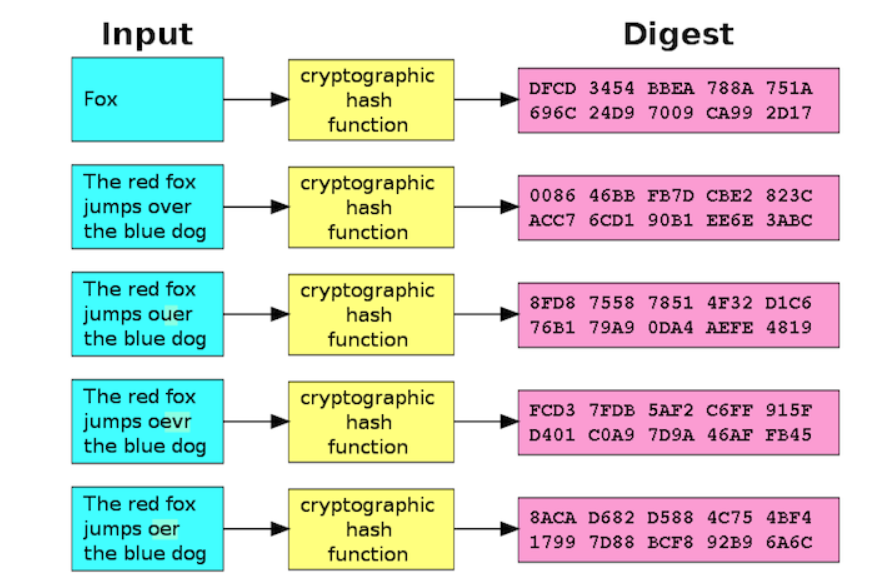
\includegraphics[width=0.99\textwidth]{funcion-hash}
\caption{Aplicación de la función hash a diferentes datos introducidos. \url{https://blog.kaspersky.com.mx/que-es-un-hash-y-como-funciona/2806/}}
\label{fig:3.1}
\end{figure}

Ahora bien, las acciones llevadas a cabo para preservar esa seguridad serían las siguientes: un usuario crea una cuenta en la aplicación, la contraseña se encripta y se almacena en la base de datos. Cuando el usuario trata de iniciar sesión y escribe la contraseña, esta se encripta y se compara el resultado con aquel que se ha guardado en la base de datos, si son iguales el usuario tendrá acceso sino, se le requerirá que lo vuelva a intentar.

El problema principal de esto es que con los avances en temas de seguridad siempre hay asociados otros que tratan de <<romper>> esa seguridad y en este caso no iba a ser menos. Creo que es importante reconocer los peligros que hay asociados a aplicar este método, pero no deseo extenderme demasiado en este aspecto así que los mencionare brevemente.


\begin{itemize}
\item Ataques de fuerza bruta. Consisten en utilizar diccionarios de palabras con contraseñas habituales e introducirlas hasta que alguna coincida. Se trata del ataque menos eficiente, pero el más difícil de evitar.
\item Tablas de búsqueda. Este tipo de ataque si que supondría un grave problema para la seguridad en el cifrado con algoritmo hash. Recordemos que las funciones hash solo se pueden encriptar, no descifrar. Lo que hace este ataque es lo siguiente, cuenta con una tabla de contraseñas típicas y su cifrado hash y las compara con los hash introducidos. Para entender mejor este concepto hay incluso herramientas online que pueden hacer este trabajo. Ver ilustración\ref{fig:3.2}. También las hay que funcionan al revés. Introduces la contraseña que crees que puede usar alguien, la encripta, la compara con todas las de la base de datos y te dice si alguien la utiliza o no.
\end{itemize}

\begin{figure}[h]
\centering
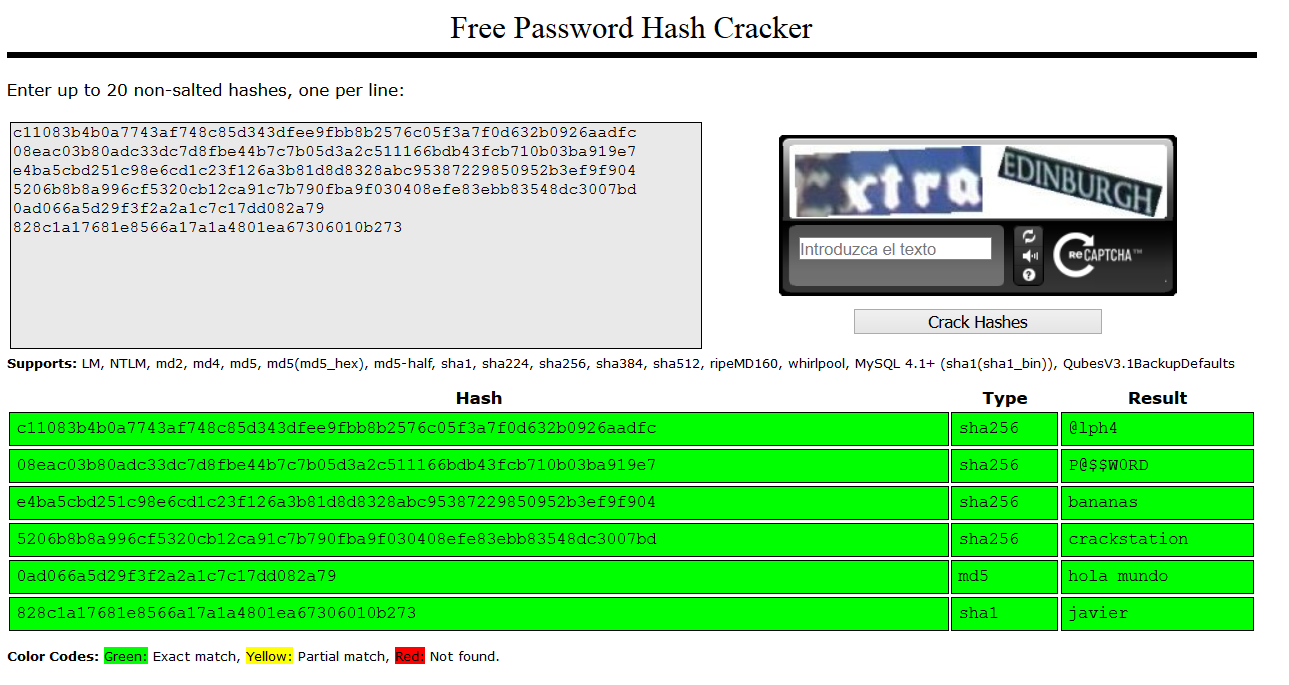
\includegraphics[width=0.99\textwidth]{hash-cracker}
\caption{Ejemplo de ataque con tablas de búsqueda. Imagen sacada de \url{https://crackstation.net/}}
\label{fig:3.2}
\end{figure}

Además de estos, hay más métodos, casi todos basados en las tablas de búsqueda. Según estos ataques queda comprobado que la seguridad de este algoritmo depende en gran mediada de la contraseña que utilice el usuario. Cuanto más aleatoria y con más mezcla de caracteres mejor, ya que formará palabras que no se encuentran en los diccionarios o tablas y solo se podrá descubrir por medio de la fuerza bruta. Entonces ¿cómo hacer que las contraseñas sean más resistentes y solucionar este problema?

Se conoce como el cifrado hash con sal o semilla. Consiste en añadir un conjunto de caracteres aleatorios, agregarlos a la contraseña y una vez hecho esto, cifrarlo con la función hash. De esta manera se consigue que la contraseña sea mucho más aleatoria que la que inicialmente ha introducido el usuario. Así podemos ver como quedaría un intento de <<tablas de búsqueda>> con este tipo de cifrado usa para contraseñas muy simples \ref{fig:3.3}. 

\begin{figure}[h]
\centering
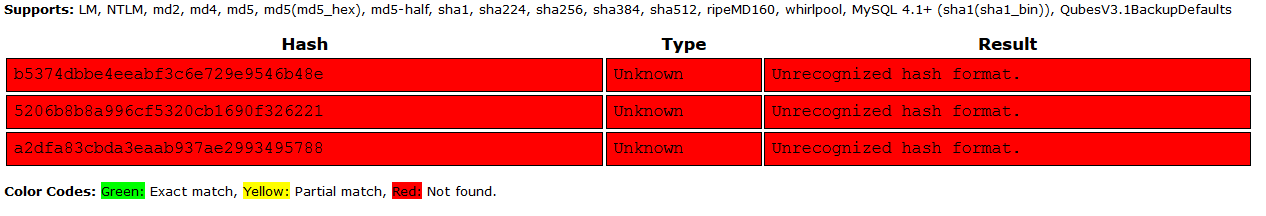
\includegraphics[width=0.99\textwidth]{hash_salt-cracker}
\caption{Resultado de aplicar tablas de búsqueda al cifrado hash con semilla. Imagen sacada de \url{https://crackstation.net/}}
\label{fig:3.3}
\end{figure}

La primera de ellas corresponde con la clave <<123>> la segunda con la palabra <<contraseña>> y la tercera con la fecha <<16-6-17>>. Todas son fáciles, pero al añadirle una clave y cifrarlo todo, se vuelve mucho mas complejo. Se podría pensar que, como la clave que se le añade también se guarda en la base de datos sigue sin ser seguro. Partiendo del hecho de que no hay prácticamente nada seguro al cien por cien, lo que se consigue con esto es dificultar mucho el cálculo, ya que los dos ataques mencionado anteriormente (y varios más basados en estos dos) se ayudan de repositorios de contraseñas. Así si quisieran descifrarlo debería de coger el conjunto aleatorio, sumarle la posible contraseña y cifrarlo comparando los resultados sólo con ese hash (o contraseña cifrada) ya que el salt es único para cada hash. Con este método se consigue que los cálculos para descifrar una contraseña sean bastante más costosos de una forma muy simple.

\capitulo{4}{Técnicas y herramientas}

Dentro de las diferentes herramientas que utilizaré para la realización de este trabajo, la más importante es aquella con la cual, realizaré la conversión a JavaScript. Es por ello esencial hacer una buena elección comparando y analizando la diferentes posibilidades a elegir.

Como principales herramientas para la conversión de Java a JavaScript he podido encontrar GWT (Google Web Toolkit), JSweet, WebSwing, Vaadin y DukeScript aunque también hay otras que descartamos por su poco relevancia o información.

\section{GWT}

Google Web Toolkit es un framework ámpliamente conocido por los desarrolladores web, entre otras cosas, gracias a ser de código abierto, de su gran utilidad y calidad además de ser completamente gratuito \footnote{\url{http://www.gwtproject.org/}}.
Contiene una SDK que proporciona un conjunto de APIs de Java que permiten el desarrollo de aplicaciones AJAX escritas en Java. Posteriormente compila el código en JavaScript ya optimizado dando robustez a la aplicación web.

Básicamente, permite a los desarrolladores compilar código JAVA en archivos JavaScript ya optimizados de forma autónoma, proporcionando así todas las ventajas de las aplicaciones escritas en este último lenguaje. 

GWT permite compartir código escrito en Java en la parte del servidor con código JavaScript en la parte del cliente lo que nos lleva pensar que la aplicación resultante será fiel a la idea inicial del Thoth. 

Nos decantamos por GWT porque, a parte de que supone un aprendizaje para mí como alumno, también es la base de otros frameworks de los que más tarde hablaré. Ha sido muy utilizado anteriormente y ahora está digamos que en decadencia. El soporte actual es mínimo y sobre todo en el tema visual anda algo anticuado. En el desarrollo del proyecto hemos llegado a ver  y probar <<bugs>> que según otros usuarios ya descubrieron hace un par de años.

Aun así, hay bastante información con la que he podido trabajar, y una comunidad grande, que aunque ahora se ha <<pasado>> a otros frameworks más actuales, han dejado huella y soluciones a muchos de los problemas con los que he trabajado.

\section{WebSwing}

En cuanto a esta herramienta, es algo diferente a las demás. WebSwing la descubrimos debido a una duda que nos surgió a al principio del proyecto. Y es que la aplicación Thoth original cuenta con muchísimos elementos de la biblioteca gráfica <<Swing>>, es digamos toda la estructura visual que utiliza. El problema surgió que con GWT no podemos hacer uso de ella ya que al ser algo visual debe ir en la parte del cliente y como ya hemos mencionado, en el cliente, que es donde se hace la traducción a JavaScript, las librerías de Java para desarrollar son muy limitadas. 

Pues bien al buscar una alternativa, descubrimos WebSwing. Se trata de un servidor web que permite la ejecución de aplicaciones que utilicen la biblioteca gráfica Swing desde el navegador, utilizando sólo HTML5. De esta forma toda la aplicación de Thoth se ejecutaría en el navegador conservando su aspecto de siempre y manteniendo las ventajas de una aplicación web.

En vez de utilizar JavaScript utiliza HTML5, cumpliendo además el objetivo principal del proyecto, que es llevar Thoth a la web.

La cuestión es que el utilizar esta herramienta no supone ningún reto como informático y facilitaría tanto el proyecto que este quedaría en nada más que unas simples mejoras de Thoth hechas con poco desarrollo. Por lo tanto la descartamos después de haberla probado.

\section{JSweet} 

JSweet\footnote{\url{http://http://www.jsweet.org/}}es básicamente un <<transpiler>> es decir un compilador que traduce un código en un lenguaje a otro lenguaje. Al igual que GWT esta orientado a objetos, que proporciona una programación segura gracias a que usa un sistema de <<tipado>> Java.

La diferencia fundamental con GWT es que al ser un <<transpiler>> hace una traducción directa entre Java y JavaScript posicionando el código a un lado o al otro del Cliente y el servidor. Esto, claramente, tiene sus ventajas y sus inconvenientes dependiendo del uso que se le quiera dar. 

porque no queriamos esto

\section{DukeScript}

Se define como una tecnología para la creación de aplicaciones Java <<multiplataforma>> que internamente hacen uso de tecnologías HTML5 y JavaScript para el renderizado.\footnote{\url{https://dukescript.com/}}
Al igual que en los casos anteriores <<sólo>> se necesita desarrollar la aplicación en Java para después transformarla. Y digo <<sólo>> porque eso es en la teoría ya que como hemos podido ver, y en parte es lógico, la traducción suele requerir, por lo menos, realizar ajustes del lenguaje para un buen funcionamiento.

DukeScript se centra sobre todo en el desarrollo de aplicaciones <<multi-plataforma>> llevadas a cabo en Java, más que en el paso de Java a JavaScript. Da la posibilidad de que alguien con conocimientos, digamoslo así, en Java pueda llevar a cabo un proyecto en lenguajes pensados para aplicaciones móviles o web. Esto no quita que se puedan realizar aplicaciones de escritorio con JavaScript.

\section{Vaadin}

Vaadin en un <<framework>> de Java de código abierto, para crear aplicaciones web \footnote{\url{https://vaadin.com/home}}. Se programa en Java o cualquier otro lenguaje de JVM. Lo mas destacado de Vaadin es que esta construido sobre una base de GWT, por ello es una de las grandes alternativas a este último. La forma de trabajar con Vaadin es mediante el lenguaje Java e incorpora un lado cliente y otro servidor, el el cual irán las funcionalidades más complejas y su programación es dirigida por eventos. Es decir, hasta aquí es igual a GWT.

Las mejoras con respecto a GWT son varias, pero voy a mencionar solo aquellas que son más relevantes para este proyecto. Cuenta sobre todo con muchos elementos visuales, mejorados y con diseños más actuales. La parte visual es tan importante en Vaadin que incluyen un <<diseñador>> o <<designer>> en inglés, en le puggin de Eclipse que facilita mucho la creación de la parte visual ya que da la posibilidad de hacer el diseño de forma visual.

En realidad la mayor parte de los elementos visuales, menús, <<boards>>, diagramas estadísticos, iconos etc, están pensados sobre todo para un uso comercial orientado sobre todo para empresas. Por ello, el problema principal es que para poder hacer uso de su potencial se necesitan licencias de pago.

Aunque cuenta con un núcleo de elementos gratuitos y periodos de prueba también gratuitos, decidimos seguir nuestro camino, por llamarlo así, con GWT y hacerlo completamente de esta forma.

\section{Herramientas para el cifrado de contraseñas}
librerias utilizadas para el cifrado, para el login etc


En este programa utilizamos una técnica muy simple, que mejora un poco este aspecto. Sabemos que existen técnicas más avanzadas que lo que hacen, sobre todo, es aumentar mucho los tiempos de procesado en los ataques por fuerza bruta por ejemplo, pero no queríamos centrarnos mucho en ese tema además de que percibimos un ralentizado a la hora de registrar a un usuario ya que cifrar la contraseña requiere un mayor tiempo de ejecución.



La técnica que empleamos es se conoce como el cifrado hash con sal o semilla (según su traducción del inglés, hashing with salt). Consiste en añadir un conjunto de caracteres aleatorio y concatenarlo a la contraseña y una vez hecho esto, cifrarlo con la función hash. De esta manera se consigue que la contraseña sea mucho más aleatoria que la que inicialmente ha introducido el usuario. Además de forma transparente para él. Para generar el salt en Java contamos con el paquete <<security>> y la clase <<SecureRandom>> especificando el tamaño del salt. 

Por otro lado, para hacer la autentificación del usuario se debe almacenar en la base de datos tanto el salt como el hash generado. Cuando el usuario introduce la contraseña para iniciar sesión, internamente se añade el salt a la contraseña introducida, se cifra con el mismo método y se comparan. Si coinciden, accederá a la aplicación, sino, deberá introducir de nuevo los datos necesarios.

tecnicas de cifrado? 
de mantenimiento de session?
subrayado con HTML?
cifrado?
\capitulo{5}{Aspectos relevantes del desarrollo del proyecto}

Lo más relevante de este proyecto es el transformar la última versión de Thoth a una aplicación web hecha por medio de GWT lo que supone comprender el funcionamiento interno del Thoth original, <<desglosándolo>> para poder adaptarlo a las condiciones de un proyecto hecho con GWT.
Estas condiciones limitan un poco la aplicación y nos obligan a reformar partes que antes eran más sencillas.

Además de condicionar Thoth a GWT, también hemos añadido nuevas funcionalidades de las que hablaremos y que completan la aplicación.



\section{Internacionalización}
La aplicación cuenta con la funcionalidad de la internacionalización. Dentro del menú se pueden elegir entre varios idiomas a los que se traducirán los diferentes elementos. Los idiomas en los que está disponible la versión web de Thoth son: Alemán, castellano o español, francés y por supuesto inglés. Consideramos que esta funcionalidad es muy importante para poder llegar a diferentes países en el caso de que fuera necesario.

La internacionalización de la aplicación es un poco diferente a la utilizada en la versión de escritorio de Thoth. En primer lugar es necesario incluir una interfaz con los métodos para la internacionalización y los mensajes <<por defecto>> asociados a cada uno. Cada vez que queramos hacer uso de esos mensajes hay que hacer una llamada al método de la interfaz. Esa interfaz se encuentra en el directorio <<client.gui.utils>> donde se encuentran también los ficheros <<properties>> asociados, donde se encuentran las diferentes traducciones según el mensaje. Estos mensajes son los mismos que los utilizados para la internacionalización de Thoth V2.

Para poder realizar el cambio de idioma es necesario hacer uso de las propiedades las clases <<xml>> y <<html>> de GWT, en concreto <<locale>> que es la que especificará la localidad, que determina el idioma. Por ello cada vez que elegimos un idioma, la aplicación se redirige a una nueva <<URL>> (llevando a cabo una nueva compilación) con el atributo \texttt{locale=} seguido de las siglas del idioma al que se quiere traducir.



\section{Cifrado de contraseñas y seguridad en Thoth Web}

El cifrado de la contraseña es una de las cuestiones más importantes para preservar la seguridad o intimidad del usuario. El porqué es muy simple. Los usuarios normalmente utilizamos las mismas contraseñas o parecidas para cualquier cuenta de una página o red social. Por lo tanto si hay alguien con acceso a la base de datos, podrá ver la contraseña utilizada por un determinado usuario poniendo en peligro esa intimidad no solo en este programa, sino, como ya se ha comentado antes, la de otras cuentas.

Para evitar esto, el método más simple es el cifrar las contraseñas en la base de datos para que en el caso en el que alguien acceda a ella, en el campo <<contraseña>> no vea la contraseña real, sino el resultado del cifrado de esta. El método de cifrado que se emplea en Thoth Web el del algoritmo <<hash>> que como veremos más adelante tiene unas características determinadas. 

\subsection{Funcionamiento del algoritmo hash}

Se trata de un algoritmo matemático con el que se transforma cualquier cantidad de datos en una serie de datos fija que funciona como una huella dactilar. Esto quiere decir que sea cual sea la cantidad de caracteres de entrada, la salida siempre será fija. Cumple además con dos premisas muy importantes para la seguridad: 

\begin{itemize}
\item No es reversible, no se puede descifrar por medio de funciones matemáticas y obtener el resultado antes de ser encriptado, sea cual sea la función utilizada (SHA-1, SHA-2 o MD 5 entre otras, como veremos a continuación).
\item Cuenta con la propiedad de que si la entrada cambia, aunque sea sólo en un bit, el hash resultante será completamente, como se puede ver en la siguiente ilustración \ref{fig:3.1}. En la imagen se puede apreciar que aunque la entrada tenga un mayor numero de caracteres, la salida siempre será de 40 caracteres.

\end{itemize} 

\begin{figure}[h]
\centering
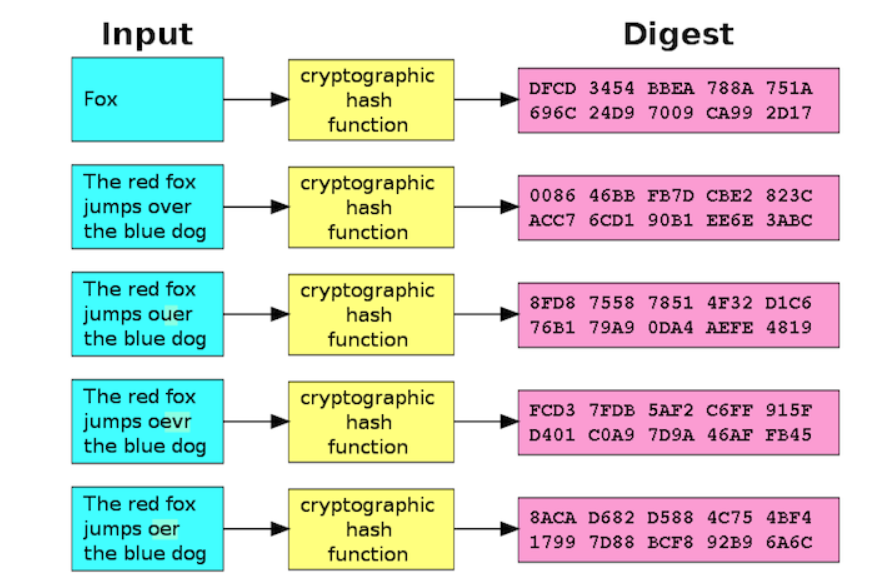
\includegraphics[width=0.99\textwidth]{funcion-hash}
\caption{Aplicación de la función hash a diferentes datos introducidos. \url{https://blog.kaspersky.com.mx/que-es-un-hash-y-como-funciona/2806/}}
\label{fig:3.1}
\end{figure}

Ahora bien, las acciones llevadas a cabo para preservar esa seguridad serían las siguientes: un usuario crea una cuenta en la aplicación, la contraseña se encripta y se almacena en la base de datos. Cuando el usuario trata de iniciar sesión y escribe la contraseña, esta se encripta y se compara el resultado con aquel que se ha guardado en la base de datos, si son iguales el usuario tendrá acceso sino, se le requerirá que lo vuelva a intentar.

El problema principal de esto es que con los avances en temas de seguridad siempre hay asociados otros que tratan de <<romper>> esa seguridad y en este caso no iba a ser menos. Creo que es importante reconocer los peligros que hay asociados a aplicar este método, pero no deseo extenderme demasiado en este aspecto así que los mencionare brevemente.


\begin{itemize}
\item Ataques de fuerza bruta. Consisten en utilizar diccionarios de palabras con contraseñas habituales e introducirlas hasta que alguna coincida. Se trata del ataque menos eficiente, pero el más difícil de evitar.
\item Tablas de búsqueda. Este tipo de ataque si que supondría un grave problema para la seguridad en el cifrado con algoritmo hash. Recordemos que las funciones hash solo se pueden encriptar, no descifrar. Lo que hace este ataque es lo siguiente, cuenta con una tabla de contraseñas típicas y su cifrado hash y las compara con los hash introducidos. Para entender mejor este concepto hay incluso herramientas online que pueden hacer este trabajo. Ver ilustración\ref{fig:3.2}. También las hay que funcionan al revés. Introduces la contraseña que crees que puede usar alguien, la encripta, la compara con todas las de la base de datos y te dice si alguien la utiliza o no.
\end{itemize}

\begin{figure}[h]
\centering
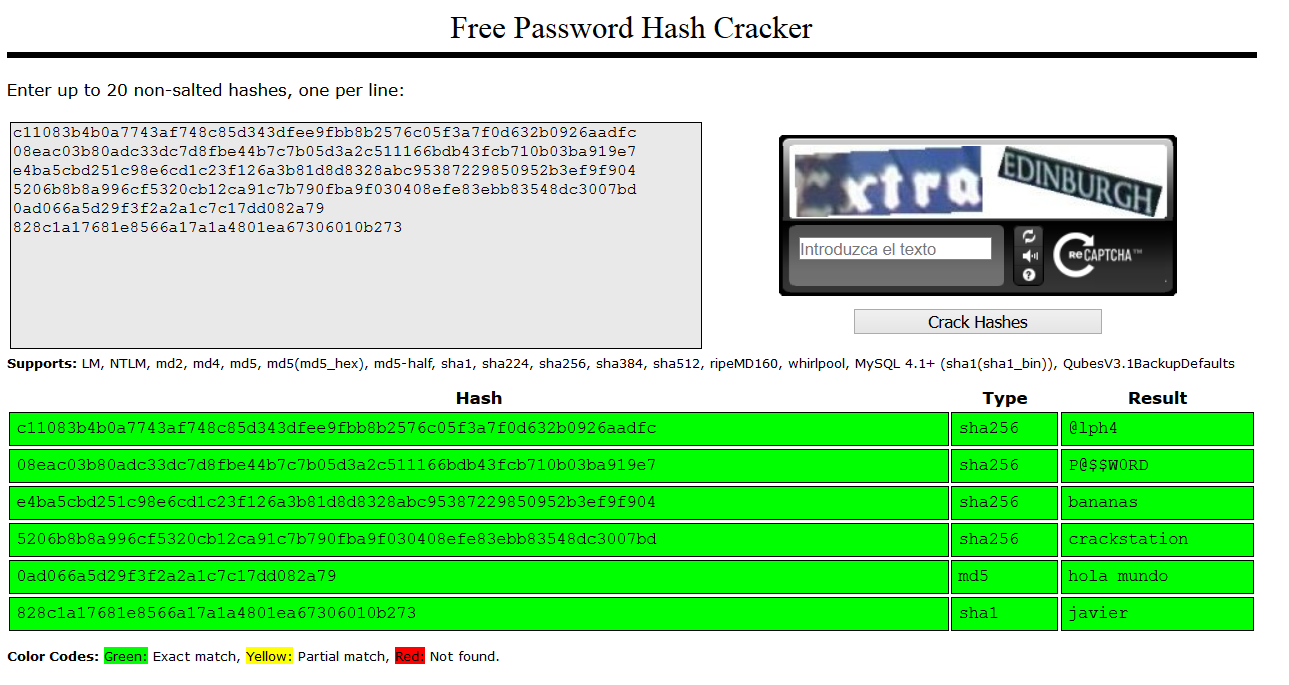
\includegraphics[width=0.99\textwidth]{hash-cracker}
\caption{Ejemplo de ataque con tablas de búsqueda. Imagen sacada de \url{https://crackstation.net/}}
\label{fig:3.2}
\end{figure}

Además de estos, hay más métodos, casi todos basados en las tablas de búsqueda. Según estos ataques queda comprobado que la seguridad de este algoritmo depende en gran mediada de la contraseña que utilice el usuario. Cuanto más aleatoria y con más mezcla de caracteres mejor, ya que formará palabras que no se encuentran en los diccionarios o tablas y solo se podrá descubrir por medio de la fuerza bruta. Entonces ¿cómo hacer que las contraseñas sean más resistentes y solucionar este problema?

Se conoce como el cifrado hash con sal o semilla. Consiste en añadir un conjunto de caracteres aleatorios, agregarlos a la contraseña y una vez hecho esto, cifrarlo con la función hash. De esta manera se consigue que la contraseña sea mucho más aleatoria que la que inicialmente ha introducido el usuario. Así podemos ver como quedaría un intento de <<tablas de búsqueda>> con este tipo de cifrado usa para contraseñas muy simples \ref{fig:3.3}. 

\begin{figure}[h]
\centering
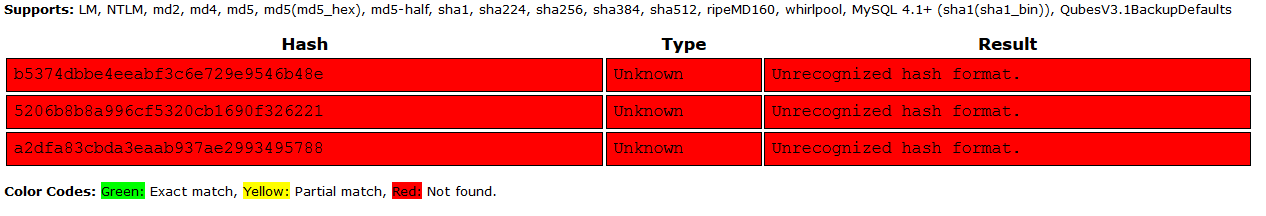
\includegraphics[width=0.99\textwidth]{hash_salt-cracker}
\caption{Resultado de aplicar tablas de búsqueda al cifrado hash con semilla. Imagen sacada de \url{https://crackstation.net/}}
\label{fig:3.3}
\end{figure}

La primera de ellas corresponde con la clave <<123>> la segunda con la palabra <<contraseña>> y la tercera con la fecha <<16-6-17>>. Todas son fáciles, pero al añadirle una clave y cifrarlo todo, se vuelve mucho mas complejo. Se podría pensar que, como la clave que se le añade también se guarda en la base de datos sigue sin ser seguro. Partiendo del hecho de que no hay prácticamente nada seguro al cien por cien, lo que se consigue con esto es dificultar mucho el cálculo, ya que los dos ataques mencionado anteriormente (y varios más basados en estos dos) se ayudan de repositorios de contraseñas. Así si quisieran descifrarlo debería de coger el conjunto aleatorio, sumarle la posible contraseña y cifrarlo comparando los resultados sólo con ese hash (o contraseña cifrada) ya que el salt es único para cada hash. Con este método se consigue que los cálculos para descifrar una contraseña sean bastante más costosos de una forma muy simple.

\section{Google Web toolkit}
Para trabajar con GWT hemos utilizado el entorno de desarrollo de eclipse y ahí 
 
 
 documentar algo del cliente serivido, que me ha costado etc.



\section{Registro e inicio de sesión de usuarios}
Todas las comunicaciones RPC, el porque utilizo modulos de carga, porque dan errores si se encuantran los modulos en las variables a ejecutar el programa.
Sobre la session y la cookies, como utilizo el gwt.xml de app engine y porque da fallo
mensaje de error sin especificar si falla el usuario o contraseña para no mostrar suficiente información como para ponerla en peligro.

\capitulo{6}{Trabajos relacionados}

En este apartado vamos a ver otros proyectos, estudios o trabajos que están relacionados con este trabajo. Explicaremos en qué consisten y qué tienen que ver con este proyecto.

\begin{itemize}

\item \textbf{Noam}: Es una biblioteca JavaScript para trabajar con autómatas y gramáticas formales para lenguajes regulares y sin contexto.

\item \textbf{JSFLAP}\footnote{\url{http://jsflap.com/}}: Se trata de una aplicación web en desarrollo, programada en JavaScript, que sirve para visualizar lenguajes formales y teoría de los autómatas. Actualmente cuenta con una versión beta, aunque su desarrollo parece que se encuentra parado. Es un programa muy visual, permite exportar un autómata en \LaTeX, en texto o en imagen o configurar el aspecto visual. Es muy útil y fácil de usar.


\item \emph{\textbf{Compiler Construction Toolkit}}\footnote{\url{http://hackingoff.com/compilers}}: Se trata de una herramienta web con la que podemos construir componentes de un compilador. Sus herramientas se pueden clasificar en
\begin{itemize}
\item Herramientas de teoría de compiladores.
\item Herramientas de diseño de compiladores.
\item Herramientas para generar un parser.
\end{itemize}
Es algo más difícil de utilizar que JSFLAP, pero cuenta con un mayor número de herramientas. Genera código en lenguaje <<Ruby>>.

\item \emph{BURGRAM}\footnote{\url{http://cgosorio.es/BURGRAM/}}: Consiste en un programa para la generación y simulación de tablas de análisis sintáctico, Dirigido por el Dr. César Ignacio García Osorio y desarrollado por Carlos Gómez Palacios.
\end{itemize}
\capitulo{7}{Conclusiones y Líneas de trabajo futuras}

En este apartado, mencionaremos algunas conclusiones a las que hemos llegado después de realizar el proyecto además de posibles ideas relacionadas con futuros proyectos.

\section{Conclusiones}

Si bien es verdad que la dirección tomada en un principio sobre qué herramienta utilizar para desarrollar el proyecto, podría haber sido más acertada, hemos aprendido mucho sobre el entorno de GWT. \emph{WebSwing} nos hubiera facilitado mucho el trabajo de transformar a HTML5 el código en Java. Pero por otro lado, hemos visto la forma en la que se desarrollan cientos de aplicaciones con GWT, algunas tan grandes como Cloudorado\footnote{\url{https://www.cloudorado.com/}}, BookedIN\footnote{\url{https://bookedin.com/}}, Gae-Studio\footnote{\url{https://dev.arcbees.com/gaestudio/}} o Sigmah\footnote{\url{http://www.sigmah.org/EN.html}}.

En el caso de que hubiéramos hecho el proyecto con herramientas más fáciles nos hubieramos centrado sobre todo en añadir mejoras de Thoth, sin perder tanto tiempo en adaptar el código Java para GWT. 

En cuanto a mi, en líneas generales, he podido aprender mucho sobre el desarrollo web, la arquitectura que utiliza y como se distribuye el programa entre el cliente y el servidor o la forma en la que se despliega una aplicación de estas características.

\section{Líneas de trabajo futuras}

Como posibles mejoras sobre este proyecto, hemos encontrado varios detalles que se nos han escapado, ya sea por falta de tiempo, o por no habernos dado cuenta antes.
\begin{itemize}
\item Creemos que es interesante almacenar en la base de datos la configuración del usuario, para que una vez que cambie el idioma de la aplicación, por defecto, al iniciar sesión lo haga con el idioma elegido anteriormente.

\item Añadir algún método para guardar y cargar gramáticas, ya sea de forma local, en ordenador del usuario, o en la base de datos.

\item poder añadir comentarios al introducir un gramática, de forma que no se tengan en cuenta a la hora de comprobar la gramática. Nos dimos cuenta tarde, al hacer varias pruebas finales.
\item Este proyecto se podría haber hecho de forma parecida pero con \emph{WebSwing} y centrándose sobre todo en la base de datos, en la accesibilidad desde distintos dispositivos etc.

\item Crear perfiles de usuario, en que pueda configurar un avatar, añadir gramáticas favoritas entre otros.

\item Añadir un panel de construcción de autómatas como en otras versiones de Thoth.
\end{itemize}


\bibliographystyle{plain}
\bibliography{bibliografia}

\end{document}
